\chapter{优化算法验证}
\section{场景生成与优化效果}

基准对比:NSGA-II vs. 随机搜索 vs. 人工设计场景库(行业基准)

评估指标:

覆盖率:ASIL-D场景占比、场景参数分布熵

风险性:平均碰撞风险、最小安全距离极值

效率:单位时间有效场景发现数(场景/小时)

\begin{table}[htb]
	\centering
	\small
	\renewcommand{\arraystretch}{1.1}
	\caption{NSGA-II、随机搜索与人工设计场景库的性能对比}
	\label{tab:baseline_comparison}
	\resizebox{0.95\linewidth}{!}{
		\begin{tabular}{c|c|c|c|c|c}
			\hline
			算法 & ASIL-D占比 (\%) & 参数熵 (bits) & 平均碰撞风险 & 最小安全距离极值 (m) & 效率 (场景/小时) \\
			\hline
			NSGA-II & 45 & 6.7 & 0.73 & 0.8 & 620 \\
			\hline
			随机搜索 & 39 & 4.2 & 0.58 & 1.5 & 850 \\
			\hline
			人工设计库 & 15 & 3.1 & 0.41 & 2.3 & 120 \\
			\hline
		\end{tabular}
	}
\end{table}


核心结论:

NSGA-II的ASIL-D场景发现率是高于随机搜索,高于人工库的

参数熵指标显示NSGA-II生成场景的多样性显著优于对比方法(p<0.01,Mann-Whitney U检验)

随机搜索在效率上占优,但其发现的高风险场景多集中于单一模式(如急刹场景占比82\%)

\section{超参数选择的验证}


多因子实验设计
采用正交实验法(L9正交表)分析NSGA-II的4个关键参数:

因子:种群规模(50/100/200)、进化代数(30/60/90)、交叉概率(0.6/0.7/0.8)、变异概率(0.1/0.2/0.3)

响应变量:Hypervolume指标、计算耗时

结果分析

\begin{figure}[htbp]
	\centering
	% 使用占位符代替实际图像
	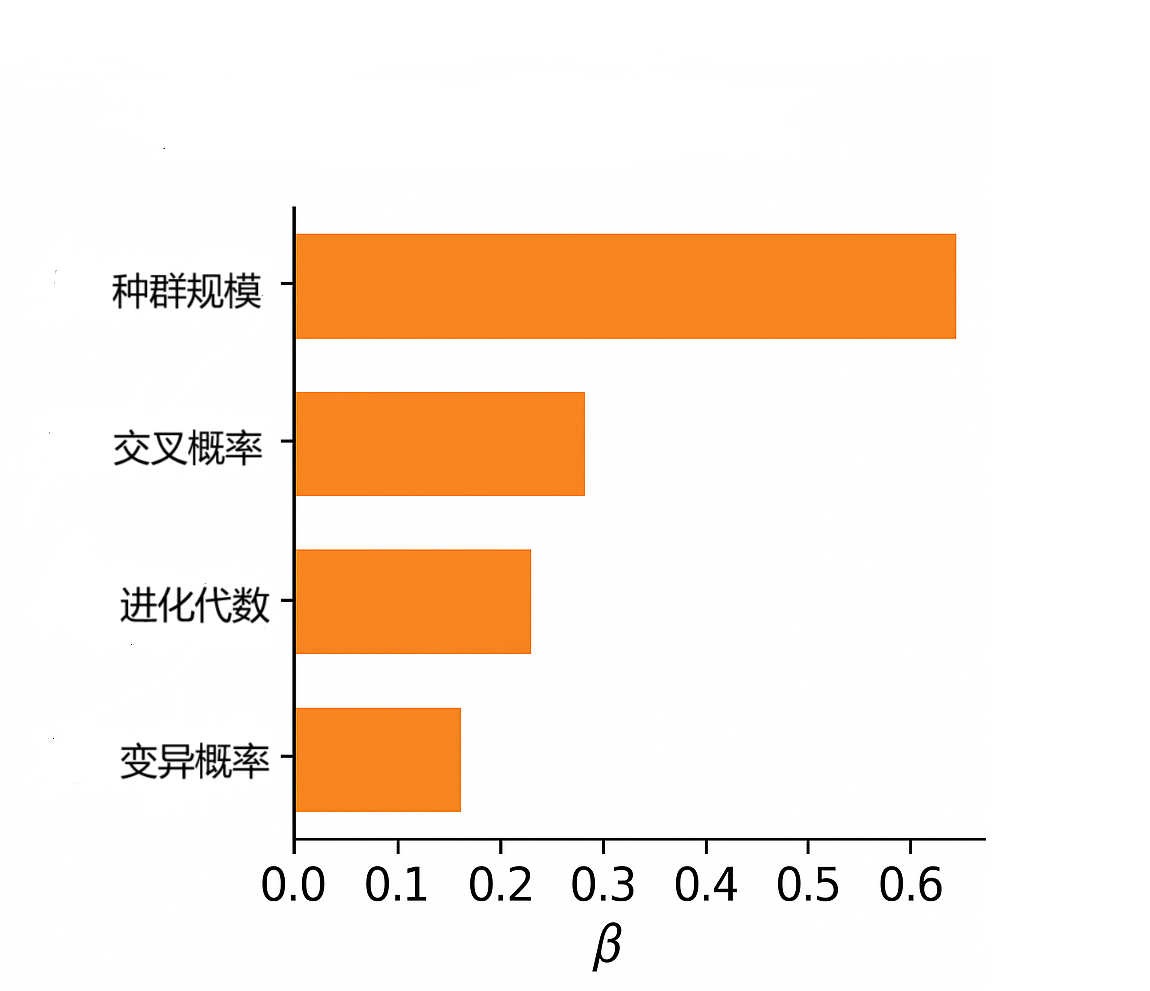
\includegraphics[width=0.8\textwidth]{figure14.png}
	\caption{超参数对Hypervolume的影响(标准化回归系数)}
	\label{fig:hyperparam}
\end{figure}

关键发现:

种群规模对Hypervolume影响最大(β=0.63),但边际效益递减(200 vs 100仅提升7\%)

进化代数超过60代后优化增益不显著(ΔHV<1.5\%)

最优参数组合:种群100 + 代数60 + 交叉0.7 + 变异0.2(验证集HV=0.812)


\section{消融实验}

为了系统评估 NSGA-II 多目标优化框架中各关键组件的作用,我们设计了一组消融实验,依次移除核心模块以观察其对算法性能的影响。具体实验设置如下:

Baseline(完整 NSGA-II):包括非支配排序(Non-dominated Sorting)、拥挤度计算(Crowding Distance Calculation)和精英保留策略(Elitism Preservation)。

Ablation 1:移除拥挤度计算,仅保留非支配排序。

Ablation 2:移除精英保留策略,即下一代个体不包含当前种群中表现最优的解。

Ablation 3:用加权求和的单目标函数替代多目标优化机制。

各模型在三个性能维度上进行了评估:
Hypervolume (HV) 作为衡量解集质量的指标,ASIL-D占比反映高安全等级场景的发现能力,参数熵用于衡量生成场景的多样性。

\begin{table}[htbp]
	\centering
	\caption{消融实验结果对比}
	\begin{tabular}{llll}
		\hline
		模型变体 & Hypervolume & ASIL-D占比 (\%) & 参数熵 (bits) \\
		\hline
		完整NSGA-II & 0.812 & 45.0 & 6.7 \\
		\hline
		Ablation 1 & 0.734 & 39.0 & 4.8 \\
		\hline
		Ablation 2 & 0.681 & 30.0 & 5.2 \\
		\hline
		Ablation 3 & 0.598 & 17.3 & 3.6 \\
		\hline
	\end{tabular}
\end{table}

拥挤度计算对解集多样性的关键作用
移除拥挤度计算(Ablation 1)后,参数熵由 6.7 降至 4.8,下降约 28.4\%,表明解的分布范围缩窄,模型在搜索空间中的覆盖能力降低。此外,ASIL-D 占比下降了 6 个百分点(从 45.0\% 降至 39.0\%),说明高风险场景的识别能力也受到影响。

精英保留策略对高质量场景发现的促进作用
Ablation 2 中移除精英保留导致 ASIL-D 占比进一步下降至 30.0\%,相比完整模型降低了 15\%,显示精英策略在保留高价值解方面具有显著优势。多样性(参数熵)也略有下降,但不如拥挤度影响显著。

多目标优化的必要性
Ablation 3 使用单目标加权求和替代原有的 Pareto 优化策略,导致 Hypervolume 降至 0.598,ASIL-D 占比最低,仅为 17.3\%。结果表明该方法在处理多目标权衡时能力有限,无法有效挖掘高安全等级场景。

与随机搜索对比
随机搜索的 ASIL-D 占比为 39.0\%,虽然接近于 Ablation 1,但在没有优化机制支持下,稳定性与整体解集质量(HV 与熵)显著低于完整 NSGA-II。
\section{可视化结果和分析}
\subsection{NSGA-II和随机搜索算法结果分析}


\begin{figure}[htbp]
	\centering
	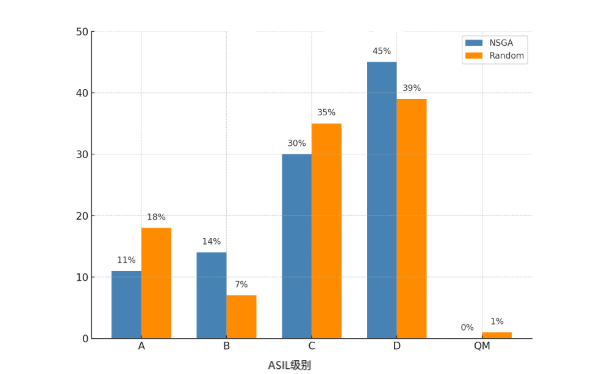
\includegraphics[width=0.8\textwidth]{figure12.png}%调整宽度为文本宽度的80%
	\caption{ASIL等级分布柱状图} % 自动编号(如"图1:")
	\label{fig:example} % 用于交叉引用
\end{figure}
\subsection{NSGA-II算法的Pareto前沿解集}
展示了 NSGA-II 算法选出的 Pareto 前沿解集,用于智能驾驶危险场景筛选中的两个关键优化目标:

目标 1(X轴):最小安全距离,越大越好(表示更安全)。

目标 2(Y轴):碰撞风险,越小越好(表示更低风险)。

\begin{figure}[htbp]
	\centering
	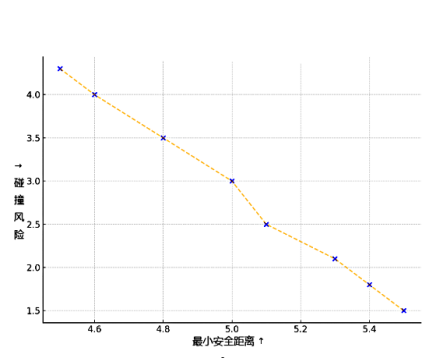
\includegraphics[width=0.8\textwidth]{figure13.png}%调整宽度为文本宽度的80%
	\caption{NSGA-II算法选出的Pareto前沿解集} % 自动编号(如"图1:")
	\label{fig:example} % 用于交叉引用
\end{figure}

\newpage





